\title{Model}

{{navbar}}

\subsubsection{Model}

A probabilistic model is a joint distribution $p(x, z)$ of data $x$
and latent variables $z$.
For more details, see the \href{/tutorials/model}{Probability Models tutorial}.
In Edward, we specify models using a simple language of random variables.

\subsubsection{Random Variables}

A random variable $\mathbf{x}$ is an object parameterized by tensors $\theta^*$.
The number of random variables in one object is determined by
the dimension of its parameters.

\begin{lstlisting}[language=Python]
from edward.models import Normal, Exponential

# univariate normal
Normal(mu=tf.constant(0.0), sigma=tf.constant(1.0))
# vector of 5 univariate normals
Normal(mu=tf.constant([0.0]*5), sigma=tf.constant([1.0]*5))
# 2 x 3 matrix of Exponentials
Exponential(lam=tf.ones([2, 3]))
\end{lstlisting}

For multivariate distributions, the multivariate dimension is the
innermost (right-most) dimension of the parameters.

\begin{lstlisting}[language=Python]
from edward.models import Dirichlet, MultivariateNormalFull

# K-dimensional Dirichlet
Dirichlet(alpha=np.array([0.1]*K)
# vector of 5 K-dimensional multivariate normals
MultivariateNormalFull(mu=tf.zeros([5, K]), sigma=...)
# 2 x 5 matrix of K-dimensional multivariate normals
MultivariateNormalFull(mu=tf.zeros([2, 5, K]), sigma=...)
\end{lstlisting}

Random variable objects are equipped with methods such as
\texttt{log_prob()}, $\log p(\mathbf{x}\mid\theta^*)$,
and \texttt{sample()}, $\mathbf{x}^*\sim p(\mathbf{x}\mid\theta^*)$.

Each object wraps a tensor $\mathbf{x}^*$, where
$\mathbf{x}^*\sim p(\mathbf{x}\mid\theta^*)$ is a sample from the
object.

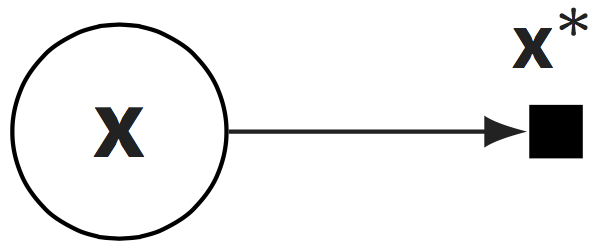
\includegraphics[width=225px]{/images/random_variable.png}

This enables operations on the TensorFlow graph, allowing random
variables to be used in conjunction with other TensorFlow ops. They
operate on $\mathbf{x}^*$.

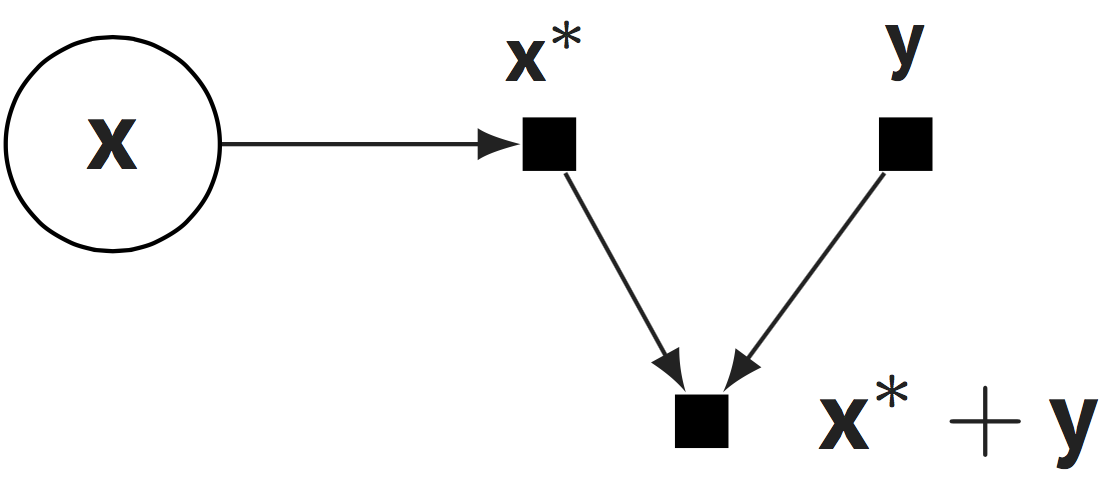
\includegraphics[width=400px]{/images/random_variable_ops.png}

\begin{lstlisting}[language=Python]
from edward.models import Normal

x = Normal(mu=tf.constant([0.0]*10), sigma=tf.constant([1.0]*10))
y = tf.constant(5.0)
x + y, x - y, x * y, x / y
tf.nn.tanh(x * y)
tf.gather(x, 2) # 3rd normal rv in the vector
\end{lstlisting}

We can leverage this construction of random variables to define
models.
For examples of models built in Edward, see the model
\href{/tutorials/}{tutorials}.

\subsubsection{Variational Models}

A variational model defines a distribution over latent variables. It
is a model of the posterior distribution, specifying another
distribution to approximate it.
Edward implements variational models using the same language of random
variables.

We parameterize them with TensorFlow variables so that their
parameters may be trained during inference.

\begin{lstlisting}[language=Python]
from edward.models import Dirichlet, Normal, InverseGamma

qpi_alpha = tf.nn.softplus(tf.Variable(tf.random_normal([K])))
qmu_mu = tf.Variable(tf.random_normal([K * D]))
qmu_sigma = tf.nn.softplus(tf.Variable(tf.random_normal([K * D])))
qsigma_alpha = tf.nn.softplus(tf.Variable(tf.random_normal([K * D])))
qsigma_beta = tf.nn.softplus(tf.Variable(tf.random_normal([K * D])))

qpi = Dirichlet(alpha=qpi_alpha)
qmu = Normal(mu=qmu_mu, sigma=qmu_sigma)
qsigma = InverseGamma(alpha=qsigma_alpha, beta=qsigma_beta)
\end{lstlisting}

{{autogenerated}}
